\documentclass[10pt,a4paper]{article}
\usepackage[T1]{fontenc}
\usepackage{newtxtext,newtxmath}
\usepackage[margin=20mm]{geometry}
\usepackage{booktabs,longtable,array}
\usepackage[authoryear,round]{natbib}
\usepackage{graphicx}
\usepackage[labelfont=bf,font=small]{caption}
\usepackage[colorlinks=true,linkcolor=black,urlcolor=blue]{hyperref}
\usepackage{xcolor}
\usepackage{placeins}
\setlength{\emergencystretch}{3em}  % long code paths break the line instead of the margin
\newcolumntype{P}[1]{>{\raggedright\arraybackslash}p{#1}}
%% Revision marking, as in main.tex (\highlighttrue marks the sections added in the revision).
\newif\ifhighlight
\highlightfalse
\definecolor{revcolor}{rgb}{0.0,0.27,0.68}
\newcommand{\revstart}{\ifhighlight\begingroup\color{revcolor}\fi}
\newcommand{\revend}{\ifhighlight\par\endgroup\fi}
%% Rows of generated tables (paper/revision_tables.py); the primitive input keeps \bottomrule working.
\makeatletter\def\inputrows#1{\@@input #1 }\makeatother
\renewcommand{\thetable}{S\arabic{table}}
\renewcommand{\thefigure}{S\arabic{figure}}
\graphicspath{{./supplementary_figs/}{./figs/}}
\setlength{\parindent}{0pt}
\setlength{\parskip}{4pt}

\begin{document}

\begin{center}
{\large\bfseries Supplementary Material}\\[2mm]
GCZ-RL: Geometry-Calibrated Residual Learning for Spinal Ligament Landmark Localization on Vertebral Surface Meshes
\end{center}

Section, equation, and table numbers without the prefix S refer to the main text. Every value in this document is regenerated by the scripts of the code release (\texttt{paper/make\_paper\_numbers.py}; for Sections S8--S13, \texttt{paper/revision\_analyses.py}, \texttt{paper/reproducibility\_check.py}, and \texttt{paper/icp\_seed\_sensitivity.py}); the mapping from each table to its script and output file is given in \texttt{docs/PAPER\_MAP.md}.

\section*{S1. Residual-regressor features}

Each GCZ point $\mathbf{p}$ of ligament class $L$ on a vertebra with vertex set $\mathcal{V}$ is described by the 36 features of Table~\ref{tab:features}. The notation is as follows. $\mathbf{v}_{\min}$ and $\mathbf{v}_{\max}$ are the componentwise minimum and maximum of $\mathcal{V}$, and $\mathbf{s}=\mathbf{v}_{\max}-\mathbf{v}_{\min}$ is the extent of the vertebra (components equal to zero are set to one). The normalized position is $\mathbf{p}_n=(\mathbf{p}-\mathbf{v}_{\min})\oslash\mathbf{s}=(x_n,y_n,z_n)$, where $\oslash$ denotes componentwise division. $\mathcal{R}_L$ is the candidate region of class $L$ used for projection (Section~3.4; if it contains fewer than two vertices, $\mathcal{V}$ is used), $\mathbf{c}_R$ its centroid, and $\mathbf{r}_{\min}$, $\mathbf{r}_{\max}$ its componentwise minimum and maximum. $[T^-_y,T^+_y]$ is the calibrated $y_n$ band of class $L$. $\bar{\mathbf{b}}_L$ is the mean normalized expert landmark centroid of class $L$ over the training vertebrae, and $\mathbf{b}=\mathbf{v}_{\min}+\bar{\mathbf{b}}_L\odot\mathbf{s}$ is its position on the current vertebra. $\mathcal{N}$ denotes the 30 vertices of $\mathcal{V}$ nearest to $\mathbf{p}$. All features are computed from the mesh, the GCZ point, and quantities learned from the training vertebrae; no annotation of the vertebra being corrected is used. Distances are in millimeters.

The features are produced by \texttt{point\_features} and \texttt{\_zone\_features} in \texttt{code/ligament/gczrl.py} of the code release. Features 5 and 6 repeat features 2 and 3; they are listed because they are part of the implemented feature vector with which all reported results were obtained. For mirrored training samples (Section~3.7), the features are computed for the mirrored point on the original mesh.

\begin{longtable}{@{}rP{38mm}P{58mm}P{48mm}@{}}
\caption{Definition of the 36 residual-regressor features.}\label{tab:features}\\
\toprule
\# & Feature & Definition & Source \\
\midrule
\endfirsthead
\toprule
\# & Feature & Definition & Source \\
\midrule
\endhead
\multicolumn{4}{@{}l}{\textit{Position of the GCZ point}}\\
1--3 & Normalized position & $x_n$, $y_n$, $z_n$ & Mesh bounding box \\
4 & Distance from mid-sagittal plane & $|x_n-0.5|$ & Mesh bounding box \\
5--6 & Normalized position (repeat) & $y_n$, $z_n$ & Mesh bounding box \\
\midrule
\multicolumn{4}{@{}l}{\textit{Relation to the candidate region}}\\
7 & Distance to region centroid & $\|\mathbf{p}-\mathbf{c}_R\|_2$ & Candidate region \\
8 & Distance to region box boundary & $\min\big(\min_k(p_k-r_{\min,k}),\ \min_k(r_{\max,k}-p_k)\big)$; positive inside the bounding box of $\mathcal{R}_L$ & Candidate region \\
9 & Relative position in $y_n$ band & $(y_n-T^-_y)/(T^+_y-T^-_y)$; 0.5 if the band is degenerate & Calibrated thresholds \\
10--12 & Normalized region centroid & $(\mathbf{c}_R-\mathbf{v}_{\min})\oslash\mathbf{s}$ & Candidate region \\
13--15 & Normalized region spread & componentwise standard deviation of $\mathcal{R}_L$, divided by $\mathbf{s}$ & Candidate region \\
16 & Region size & number of vertices in $\mathcal{R}_L$ & Candidate region \\
17--19 & Region shape & singular values $\sigma_1,\sigma_2,\sigma_3$ of the centered vertices of $\mathcal{R}_L$, divided by $\sigma_1+\sigma_2+\sigma_3$ & Candidate region \\
\midrule
\multicolumn{4}{@{}l}{\textit{Anatomical context}}\\
20 & Vertebral level & index of the level in the order C1--C7, T1--T13, L1--L5, divided by 24 & Level label \\
21--27 & Ligament class & one-hot encoding of ALL, PLL, LF, ISL, SSL, ITL, CL & Class label \\
\midrule
\multicolumn{4}{@{}l}{\textit{Local surface}}\\
28--30 & Surface normal & right singular vector of the smallest singular value of the centered set $\mathcal{N}$ (unit length) & Mesh, 30 nearest vertices \\
31 & Surface variation & $\sigma_3/(\sigma_1+\sigma_2+\sigma_3)$ of the centered set $\mathcal{N}$ & Mesh, 30 nearest vertices \\
32 & Signed lateral position & $x_n-0.5$ & Mesh bounding box \\
\midrule
\multicolumn{4}{@{}l}{\textit{Offset from the training prior}}\\
33 & Distance to class prior & $\|\mathbf{p}-\mathbf{b}\|_2$ & Training annotations (class mean) \\
34--36 & Direction to class prior & $(\mathbf{b}-\mathbf{p})\oslash\mathbf{s}$ & Training annotations (class mean) \\
\bottomrule
\end{longtable}

\section*{S2. Candidate-region construction}

For class $L$, three normalized quantities are calibrated: $y_n$, $|x_n-0.5|$, and $z_n$. For each, the mean $\mu_L$ and sample standard deviation $\sigma_L$ of the expert landmarks of the training vertebrae, normalized within their own vertebra, give the band $[\mu_L-k_L\sigma_L,\ \mu_L+k_L\sigma_L]$ with $k_L=2$, clipped to $[0,1]$ (Eq.~3). The candidate region is the set of mesh vertices that lie inside all three bands. If fewer than 64 vertices remain, the $z_n$ band is dropped and the region is formed from the $y_n$ and $|x_n-0.5|$ bands; in the GCZ selection step, if fewer than 64 vertices still remain, only the $y_n$ band is used. If no vertex satisfies the bands, the whole mesh is used. These rules are implemented in \texttt{build\_thresholds} and \texttt{candidate\_vertices} of \texttt{code/ligament/gcz.py}.

\section*{S3. Point accounting and matching-independent metrics}

The following statistics refer to the primary, patient-level leave-one-subject-out evaluation (14 lumbar vertebrae, 98 vertebra--class cases) and are computed from the saved predictions and annotations of the code release; no model was retrained. The expert annotations are dense point sets along each attachment footprint, whereas GCZ and GCZ-RL output ten landmarks per class (one for SSL and two for ITL) and SLD a class-dependent number. One-to-one Hungarian matching within each vertebra--class case pairs $\min(|P|,|G|)$ points; in every case the predicted set was the smaller one, so every predicted landmark was paired and no predicted landmark was left unpaired. No method had a missing output for any case.

\begin{table}[h]
\centering
\small
\caption{Point accounting of the primary evaluation. Ref.: number of expert reference points. Pred.: number of predicted landmarks, all of which were matched. Cov.: matched reference points as a percentage of all reference points. Unpaired reference points are Ref.\ minus Pred.}
\label{tab:accounting}
\begin{tabular}{@{}lrrrrrrr@{}}
\toprule
 & & \multicolumn{2}{c}{GCZ} & \multicolumn{2}{c}{GCZ-RL} & \multicolumn{2}{c}{SLD} \\
\cmidrule(lr){3-4}\cmidrule(lr){5-6}\cmidrule(lr){7-8}
 & Ref. & Pred. & Cov.\% & Pred. & Cov.\% & Pred. & Cov.\% \\
\midrule
\multicolumn{8}{@{}l}{\textit{By class}} \\
ALL & 368 & 140 & 38.0 & 140 & 38.0 & 196 & 53.3 \\
PLL & 239 & 140 & 58.6 & 140 & 58.6 & 196 & 82.0 \\
LF & 349 & 140 & 40.1 & 140 & 40.1 & 132 & 37.8 \\
ISL & 330 & 140 & 42.4 & 140 & 42.4 & 196 & 59.4 \\
SSL & 14 & 14 & 100.0 & 14 & 100.0 & 14 & 100.0 \\
ITL & 28 & 28 & 100.0 & 28 & 100.0 & 28 & 100.0 \\
CL & 837 & 140 & 16.7 & 140 & 16.7 & 176 & 21.0 \\
\midrule
\multicolumn{8}{@{}l}{\textit{By held-out subject}} \\
S01 & 1020 & 265 & 26.0 & 265 & 26.0 & 337 & 33.0 \\
S02 & 564 & 212 & 37.6 & 212 & 37.6 & 264 & 46.8 \\
S03 & 581 & 265 & 45.6 & 265 & 45.6 & 337 & 58.0 \\
\midrule
\textbf{All} & 2165 & 742 & 34.3 & 742 & 34.3 & 938 & 43.3 \\
\bottomrule
\end{tabular}
\end{table}

Because matched-pair metrics do not penalize reference points without a prediction, Table~\ref{tab:indep} reports metrics that use every predicted and every reference point and do not depend on matching. The closest-point distance from predictions to references (P$\rightarrow$R) is the mean, over predicted landmarks, of the distance to the nearest reference point; it is the error definition of \citet{blomenkamp2026sld} and is never larger than the matched MAE. The closest-point distance from references to predictions (R$\rightarrow$P) is the mean, over reference points, of the distance to the nearest prediction; it penalizes parts of the footprint that no prediction covers. The symmetric distance is the mean of the two, and the last block is the percentage of all reference points whose nearest prediction lies within 5~mm.

\begin{table}[h]
\centering
\small
\caption{Matching-independent metrics of the primary evaluation, averaged over the vertebra--class cases of each class; the last row averages over all 98 cases (equal to the macro average, since every class has 14 cases). Lowest distance and highest percentage per row and block in bold.}
\label{tab:indep}
\resizebox{\textwidth}{!}{%
\begin{tabular}{@{}lrrrrrrrrrrrr@{}}
\toprule
 & \multicolumn{3}{c}{P$\rightarrow$R closest point (mm)} & \multicolumn{3}{c}{R$\rightarrow$P closest point (mm)} & \multicolumn{3}{c}{Symmetric (mm)} & \multicolumn{3}{c}{Reference points within 5~mm (\%)} \\
\cmidrule(lr){2-4}\cmidrule(lr){5-7}\cmidrule(lr){8-10}\cmidrule(lr){11-13}
Class & GCZ & GCZ-RL & SLD & GCZ & GCZ-RL & SLD & GCZ & GCZ-RL & SLD & GCZ & GCZ-RL & SLD \\
\midrule
ALL & 2.605 & 2.382 & \textbf{1.521} & 3.989 & 3.798 & \textbf{3.175} & 3.297 & 3.090 & \textbf{2.348} & 70.5 & 75.4 & \textbf{78.4} \\
PLL & 1.846 & 1.846 & \textbf{1.177} & 2.329 & 2.329 & \textbf{1.969} & 2.087 & 2.087 & \textbf{1.573} & \textbf{97.2} & \textbf{97.2} & 92.3 \\
LF & 1.918 & \textbf{1.912} & 4.015 & 3.334 & \textbf{3.323} & 9.829 & 2.626 & \textbf{2.618} & 6.922 & \textbf{80.8} & \textbf{80.8} & 34.3 \\
ISL & 2.262 & 2.173 & \textbf{1.367} & 3.706 & 3.621 & \textbf{3.143} & 2.984 & 2.897 & \textbf{2.255} & 77.0 & 77.3 & \textbf{82.1} \\
SSL & 2.917 & 2.692 & \textbf{1.968} & 2.917 & 2.692 & \textbf{1.968} & 2.917 & 2.692 & \textbf{1.968} & 78.6 & 78.6 & \textbf{92.9} \\
ITL & 6.262 & 1.796 & \textbf{0.873} & 6.262 & 1.796 & \textbf{0.873} & 6.262 & 1.796 & \textbf{0.873} & 53.6 & 92.9 & \textbf{100.0} \\
CL & 2.302 & 2.180 & \textbf{1.591} & 5.631 & \textbf{5.522} & 7.664 & 3.966 & \textbf{3.851} & 4.628 & 46.8 & 46.9 & \textbf{63.4} \\
\midrule
Mean over cases & 2.873 & 2.140 & \textbf{1.787} & 4.024 & \textbf{3.297} & 4.089 & 3.448 & \textbf{2.719} & 2.938 & 72.1 & \textbf{78.4} & 77.6 \\
\bottomrule
\end{tabular}}
\end{table}

\section*{S4. Candidate-region feasibility}

For each outer fold of the primary evaluation, the candidate regions of the held-out vertebrae were rebuilt from the training subjects exactly as in the method (Section~S2), and each reference landmark of the held-out subject was assigned to the mesh vertex nearest to it. A landmark counts as inside if that vertex belongs to the region of its class. The GCZ selection step and the GCZ-RL projection step use the same bands but differ in their last fallback (Section~S2); they produce identical regions for every class except ITL. By vertebral level, the percentage of reference landmarks inside their region was L1 87.5\%, L2 96.9\%, L3 95.1\%, L4 89.5\%, L5 76.2\%.

\begin{table}[h]
\centering
\small
\caption{Candidate-region feasibility on the held-out vertebrae of the primary evaluation (14 vertebrae per class). Inside: reference landmarks whose nearest mesh vertex lies in the region of their class. Region size: median number of vertices (meshes have a median of 33{,}445 vertices). Fallback: cases in which fewer than 64 vertices satisfied all three bands. Side empty: ITL or CL cases in which the projection region had no vertex on one side of the mid-sagittal plane.}
\label{tab:zones}
\begin{tabular}{@{}lrrrrrrr@{}}
\toprule
 & & & \multicolumn{2}{c}{Region size} & \multicolumn{2}{c}{Fallback} & \\
\cmidrule(lr){4-5}\cmidrule(lr){6-7}
Class & Ref. & Inside\% & Selection & Projection & Selection & Projection & Side empty \\
\midrule
ALL & 368 & 96.7 & 6041 & 6041 & 0/14 & 0/14 & 0 \\
PLL & 239 & 83.7 & 2891 & 2891 & 0/14 & 0/14 & 0 \\
LF & 349 & 87.4 & 5254.5 & 5254.5 & 0/14 & 0/14 & 0 \\
ISL & 330 & 94.5 & 2764 & 2764 & 0/14 & 0/14 & 0 \\
SSL & 14 & 85.7 & 124.5 & 124.5 & 5/14 & 5/14 & 0 \\
ITL & 28 & 92.9 & 10990 & 34.5 & 14/14 & 14/14 & 2 \\
CL & 837 & 88.1 & 8467.5 & 8467.5 & 0/14 & 0/14 & 0 \\
\midrule
\textbf{All} & 2165 & 90.0 & -- & -- & 19/98 & 19/98 & 2 \\
\bottomrule
\end{tabular}
\end{table}

The two side-empty cases are the two ITL vertebrae (S01 L5 and S02 L4) for which the corrected point keeps its GCZ position (Section~4.3).

\section*{S5. Implementation details and hyperparameters}

Table~\ref{tab:hyper} lists the settings of every component. All are fixed; none was tuned on held-out annotations except the per-class development configuration (Section~3.7), whose selection after inspection of held-out outputs is disclosed in the main text.

\begin{longtable}{@{}P{40mm}P{118mm}@{}}
\caption{Implementation settings.}\label{tab:hyper}\\
\toprule
Component & Setting \\
\midrule
\endfirsthead
\toprule
Component & Setting \\
\midrule
\endhead
Candidate regions & $k_L=2$; bands clipped to $[0,1]$; fallback below 64 vertices (Section~S2). \\
Atlas selection & ICP from every atlas vertebra, 1200 sampled atlas points, at most 40 iterations, tolerance $10^{-5}$; residual = mean nearest-neighbor distance of 1200 sampled atlas points. \\
Full alignment & ICP, 5000 sampled points, at most 150 iterations, tolerance $10^{-6}$ (primary evaluation and development GCZ column) or $10^{-5}$ (development GCZ-RL input). \\
GCZ selection & Snap radius 15~mm; left/right split for LF and ITL, four quadrants for CL; farthest-point sampling to ten landmarks. A fallback landmark template pooled from all training vertebrae is used only if the selected atlas lacks a class. \\
Residual targets & Hungarian pairing of GCZ and expert points; mirroring of LF, ISL, ITL, CL about the sagittal plane through the vertex centroid. \\
Correction bound & $\tau_L$ = mean + 2 SD of training residual magnitudes of class $L$ (including mirrored samples). \\
Extra Trees ET-1 & 220 trees, maximum depth 18, minimum leaf size 1, 85\% of features per split, no bootstrap, seed 8. \\
Extra Trees ET-2 & 520 trees, unlimited depth, minimum leaf size 1, all features, no bootstrap, seed 91. \\
Extra Trees ET-3 & 520 trees, maximum depth 13, minimum leaf size 2, 75\% of features, no bootstrap, seed 92. \\
Extra Trees ET-4 & 520 trees, maximum depth 18, minimum leaf size 1, 85\% of features, bootstrap, seed 93. \\
Other regressors (Table~3) & Ridge ($\lambda=25$, standardized features); $k$-nearest neighbors ($k=\min(31,\max(5,\lfloor\sqrt{n}\rfloor))$, distance-weighted, standardized); random forest (420 trees, 85\% of features, bootstrap, seed 94); gradient boosting (260 trees, learning rate 0.035, depth 3, subsample 0.85, seed 95) and histogram gradient boosting (260 iterations, learning rate 0.035, 31 leaves, L2 0.05, seed 96), each with one model per output coordinate. \\
Development configuration & ALL ET-2, $\alpha=1.20$; PLL ET-2, 1.20; LF ET-1, 1.00; ISL ET-4, 1.20; SSL ET-1, 1.00; ITL ET-4, 1.00; CL ET-2, 1.10. \\
Primary selection grid & ET-1 to ET-4 $\times$ $\alpha\in\{0,0.25,0.40,0.55,0.70,0.85,1.00,1.10,1.20\}$ per class and fold, inner leave-one-subject-out; ties broken by configuration name, then $\alpha$ (Table~\ref{tab:selected}). \\
SLD & Released SpineLib code (commit 62f39cf); pyACVD remeshing (subdivision 3, 5000 clusters), 10 smoothing iterations, hole filling up to 1000, \texttt{Spine(max\_angle=60)}, shape decomposition without lamina; landmarks snapped to the input mesh; LPS$\leftrightarrow$RAS conversion; centerline approximated by cross-section centroids. \\
Software & Python 3.11, NumPy 2.4, SciPy 1.17, pandas 3.0, scikit-learn 1.8, trimesh 4.12, VTK 9.6, PyVista 0.47, pyACVD 0.4. \\
\bottomrule
\end{longtable}

\paragraph{Sensitivity of the atlas selection to the computing environment} The reported results use the ICP alignments stored with the code release, from which every number is regenerated exactly. When all alignments of the primary evaluation were recomputed from scratch in a second computing environment (same code, same pinned library versions, and the same input files, verified by checksum), the selected atlas vertebra changed for 2 of the 14 held-out vertebrae (S01 L3 and S02 L3), and the changed training-side predictions altered the inner model selection of the S01 and S02 folds. The macro-averaged MAE became 3.208~mm for GCZ and 2.418~mm for GCZ-RL (Pass@5 83.1\% and 89.8\%); SLD, which does not use ICP, was unchanged at 2.224~mm. The S03 fold was unchanged. Most of the difference comes from S02 L3, for which the newly selected atlas had a lower quick-ICP residual (1.33 against 1.51~mm) but a GCZ error higher by 4.0~mm, that is, an alignment with a small surface distance but wrong correspondence. The improvement of GCZ-RL over GCZ (24.6\%) is preserved, whereas the ordering of GCZ-RL and SLD by macro-averaged MAE is not. Atlas selection starts ICP from the scanner coordinates of each vertebra, and several candidate alignments converge to local minima with residuals of 4--5~mm; the selection is therefore sensitive to small numerical differences. \revstart A systematic analysis over ten ICP seeds is given in Section~S13.\revend

\paragraph{Correction of the calibration regressor comparison} The leave-one-vertebra-out comparison of Table~3 evaluates, for each held-out calibration vertebra, the corrections predicted for its GCZ points. In the version reported in the first author's dissertation, the validation rows of the bilateral classes (LF, ISL, ITL, CL) were taken as the first $n$ rows of that vertebra and class, where $n$ is its number of GCZ points; because original and mirrored samples alternate, half of these rows were mirrored samples, and their predicted corrections were applied to the wrong GCZ points. In addition, zones, class prior, and correction bound were computed once from all 20 calibration vertebrae. Table~\ref{tab:regcorr} compares the published values with the corrected protocol used in Table~3, in which only original samples are validated, each with its own GCZ point, and zones, prior, and bound are recomputed without the held-out vertebra. The correction lowers the errors of LF, ISL, and CL for every family; for ITL the corrected errors are 0.16--0.44~mm higher, mainly because zones, class prior, and correction bound no longer include the held-out vertebra. Under the corrected protocol Extra Trees is the best family for every class; the conclusion that Extra Trees is the most suitable residual regressor is unchanged. The development configuration had been fixed before the correction and is unchanged.

\begin{table}[h]
\centering
\small
\caption{Mean over classes of the leave-one-vertebra-out calibration MAE (mm) under the published and corrected protocols, and the MAE of the bilateral classes under the corrected protocol (published values in parentheses).}
\label{tab:regcorr}
\resizebox{\textwidth}{!}{%
\begin{tabular}{@{}lrrrrr@{}}
\toprule
 & Ridge & KNN & Random forest & Gradient boosting & Extra Trees \\
\midrule
Mean, published protocol & 3.103 & 3.017 & 2.754 & 2.774 & 2.575 \\
Mean, validation rows corrected & 2.986 & 2.655 & 2.241 & 2.274 & 1.984 \\
Mean, rows and fold quantities corrected (Table~3) & 3.055 & 2.715 & 2.307 & 2.337 & 2.037 \\
\midrule
LF & 3.546 (3.760) & 2.744 (3.653) & 2.448 (3.329) & 2.386 (3.545) & 2.125 (3.354) \\
ISL & 1.981 (2.013) & 1.918 (1.945) & 1.588 (1.831) & 1.622 (1.918) & 1.551 (1.805) \\
ITL & 4.046 (3.816) & 4.085 (3.833) & 3.399 (3.097) & 3.532 (3.090) & 3.170 (3.014) \\
CL & 4.817 (5.214) & 3.700 (5.214) & 2.934 (5.386) & 2.963 (5.128) & 2.578 (5.049) \\
\bottomrule
\end{tabular}}
\end{table}

\section*{S6. Diagnostic analysis of the correspondence rule}

Pure Hungarian matching minimizes the total distance but can pair anatomically non-corresponding points, such as left--right swaps, superior--inferior inversions, and long jumps along curved attachment regions. To quantify this, an anatomy-constrained correspondence was evaluated for a geometry-only GCZ prediction on the nine held-out lumbar vertebrae of the development analysis with complete landmark sets (S02 L1--L4 and S03 L1--L5): ALL and PLL used side-aware matching with a superior--inferior band, LF and ITL strict left--right constraints, CL a four-quadrant strategy, and ISL and SSL local ordering and distance constraints; pairs that violated these rules were penalized or rejected.

\textit{Important difference from the main evaluation.} In this diagnostic, which was run with the original analysis notebook, the number of GCZ landmarks per class was set to the number of reference points of the evaluated vertebra (at least four), so that nearly every reference point could be paired. This uses the cardinality, though not the positions, of the evaluated annotations. The analysis therefore characterizes the matching rules only. Its predictions are not those evaluated in the main text, which use a fixed number of at most ten landmarks per class, and its values are not comparable with the evaluation tables of the main text.

The nine vertebrae carry 1145 reference landmarks. Pure Hungarian matching paired 1126 of them (coverage 98.3\%), whereas the constrained rules, which leave a landmark unpaired when no admissible candidate exists, paired 1039 (90.7\%) and 1042 (91.0\%). At this lower coverage, the final constrained rule had an MAE of 3.67~mm against 4.85~mm, an RMSE of 5.34~mm against 7.71~mm, a pass rate of 82.2\% against 75.2\%, and 58 instead of 119 errors above 10~mm (Table~\ref{tab:matching_versions}, Fig.~\ref{fig:matching_versions}). The error statistics of the three rows are computed over different sets of pairs and are not directly comparable, and part of the improvement may come from landmarks that the constrained rules leave unpaired. The analysis supports the narrower conclusion that anatomical constraints remove long-range mispairings. Table~\ref{tab:per_ligament} reports the per-ligament MAE under the initial and final rules. The largest change was for ALL, from 5.07 to 4.17~mm, after side-aware and superior--inferior band constraints; PLL improved slightly. The other classes kept the initial rule, because further band, principal-axis, and ordering variants did not improve the balance between MAE, pass rate, and long errors.

\begin{table}[h]
\centering
\small
\caption{Pooled metrics of the diagnostic geometry-only GCZ prediction under three correspondence strategies (nine held-out lumbar vertebrae, 1145 reference landmarks). Coverage: paired reference landmarks as a percentage of all reference landmarks. Rows are computed over different sets of pairs. $N>10$: pairs with an error above 10~mm.}
\label{tab:matching_versions}
\begin{tabular}{@{}lrrrrrrr@{}}
\toprule
Correspondence strategy & Pairs & Cov.\% & MAE & SD & RMSE & Pass\% & $N>10$ \\
\midrule
Pure Euclidean Hungarian & 1126 & 98.3 & 4.85 & 5.99 & 7.71 & 75.2 & 119 \\
Initial anatomy-aware matching & 1039 & 90.7 & 3.84 & 4.30 & 5.76 & 80.2 & 61 \\
Final anatomy-constrained & 1042 & 91.0 & 3.67 & 3.87 & 5.34 & 82.2 & 58 \\
\bottomrule
\end{tabular}
\end{table}

\begin{table}[h]
\centering
\small
\caption{Per-ligament MAE (mm) of the diagnostic geometry-only GCZ prediction under the initial and final correspondence rules (nine held-out lumbar vertebrae).}
\label{tab:per_ligament}
\begin{tabular}{@{}lrrr@{}}
\toprule
Lig. & Initial MAE & Final MAE & $N>10$ \\
\midrule
ALL & 5.07 & 4.17 & 13 \\
PLL & 3.70 & 3.62 & 3 \\
LF  & 3.21 & 3.21 & 14 \\
ISL & 4.43 & 4.43 & 15 \\
SSL & 1.86 & 1.86 & 0 \\
ITL & 2.68 & 2.68 & 0 \\
CL  & 3.36 & 3.36 & 13 \\
\bottomrule
\end{tabular}
\end{table}

\begin{figure}[h]
\centering
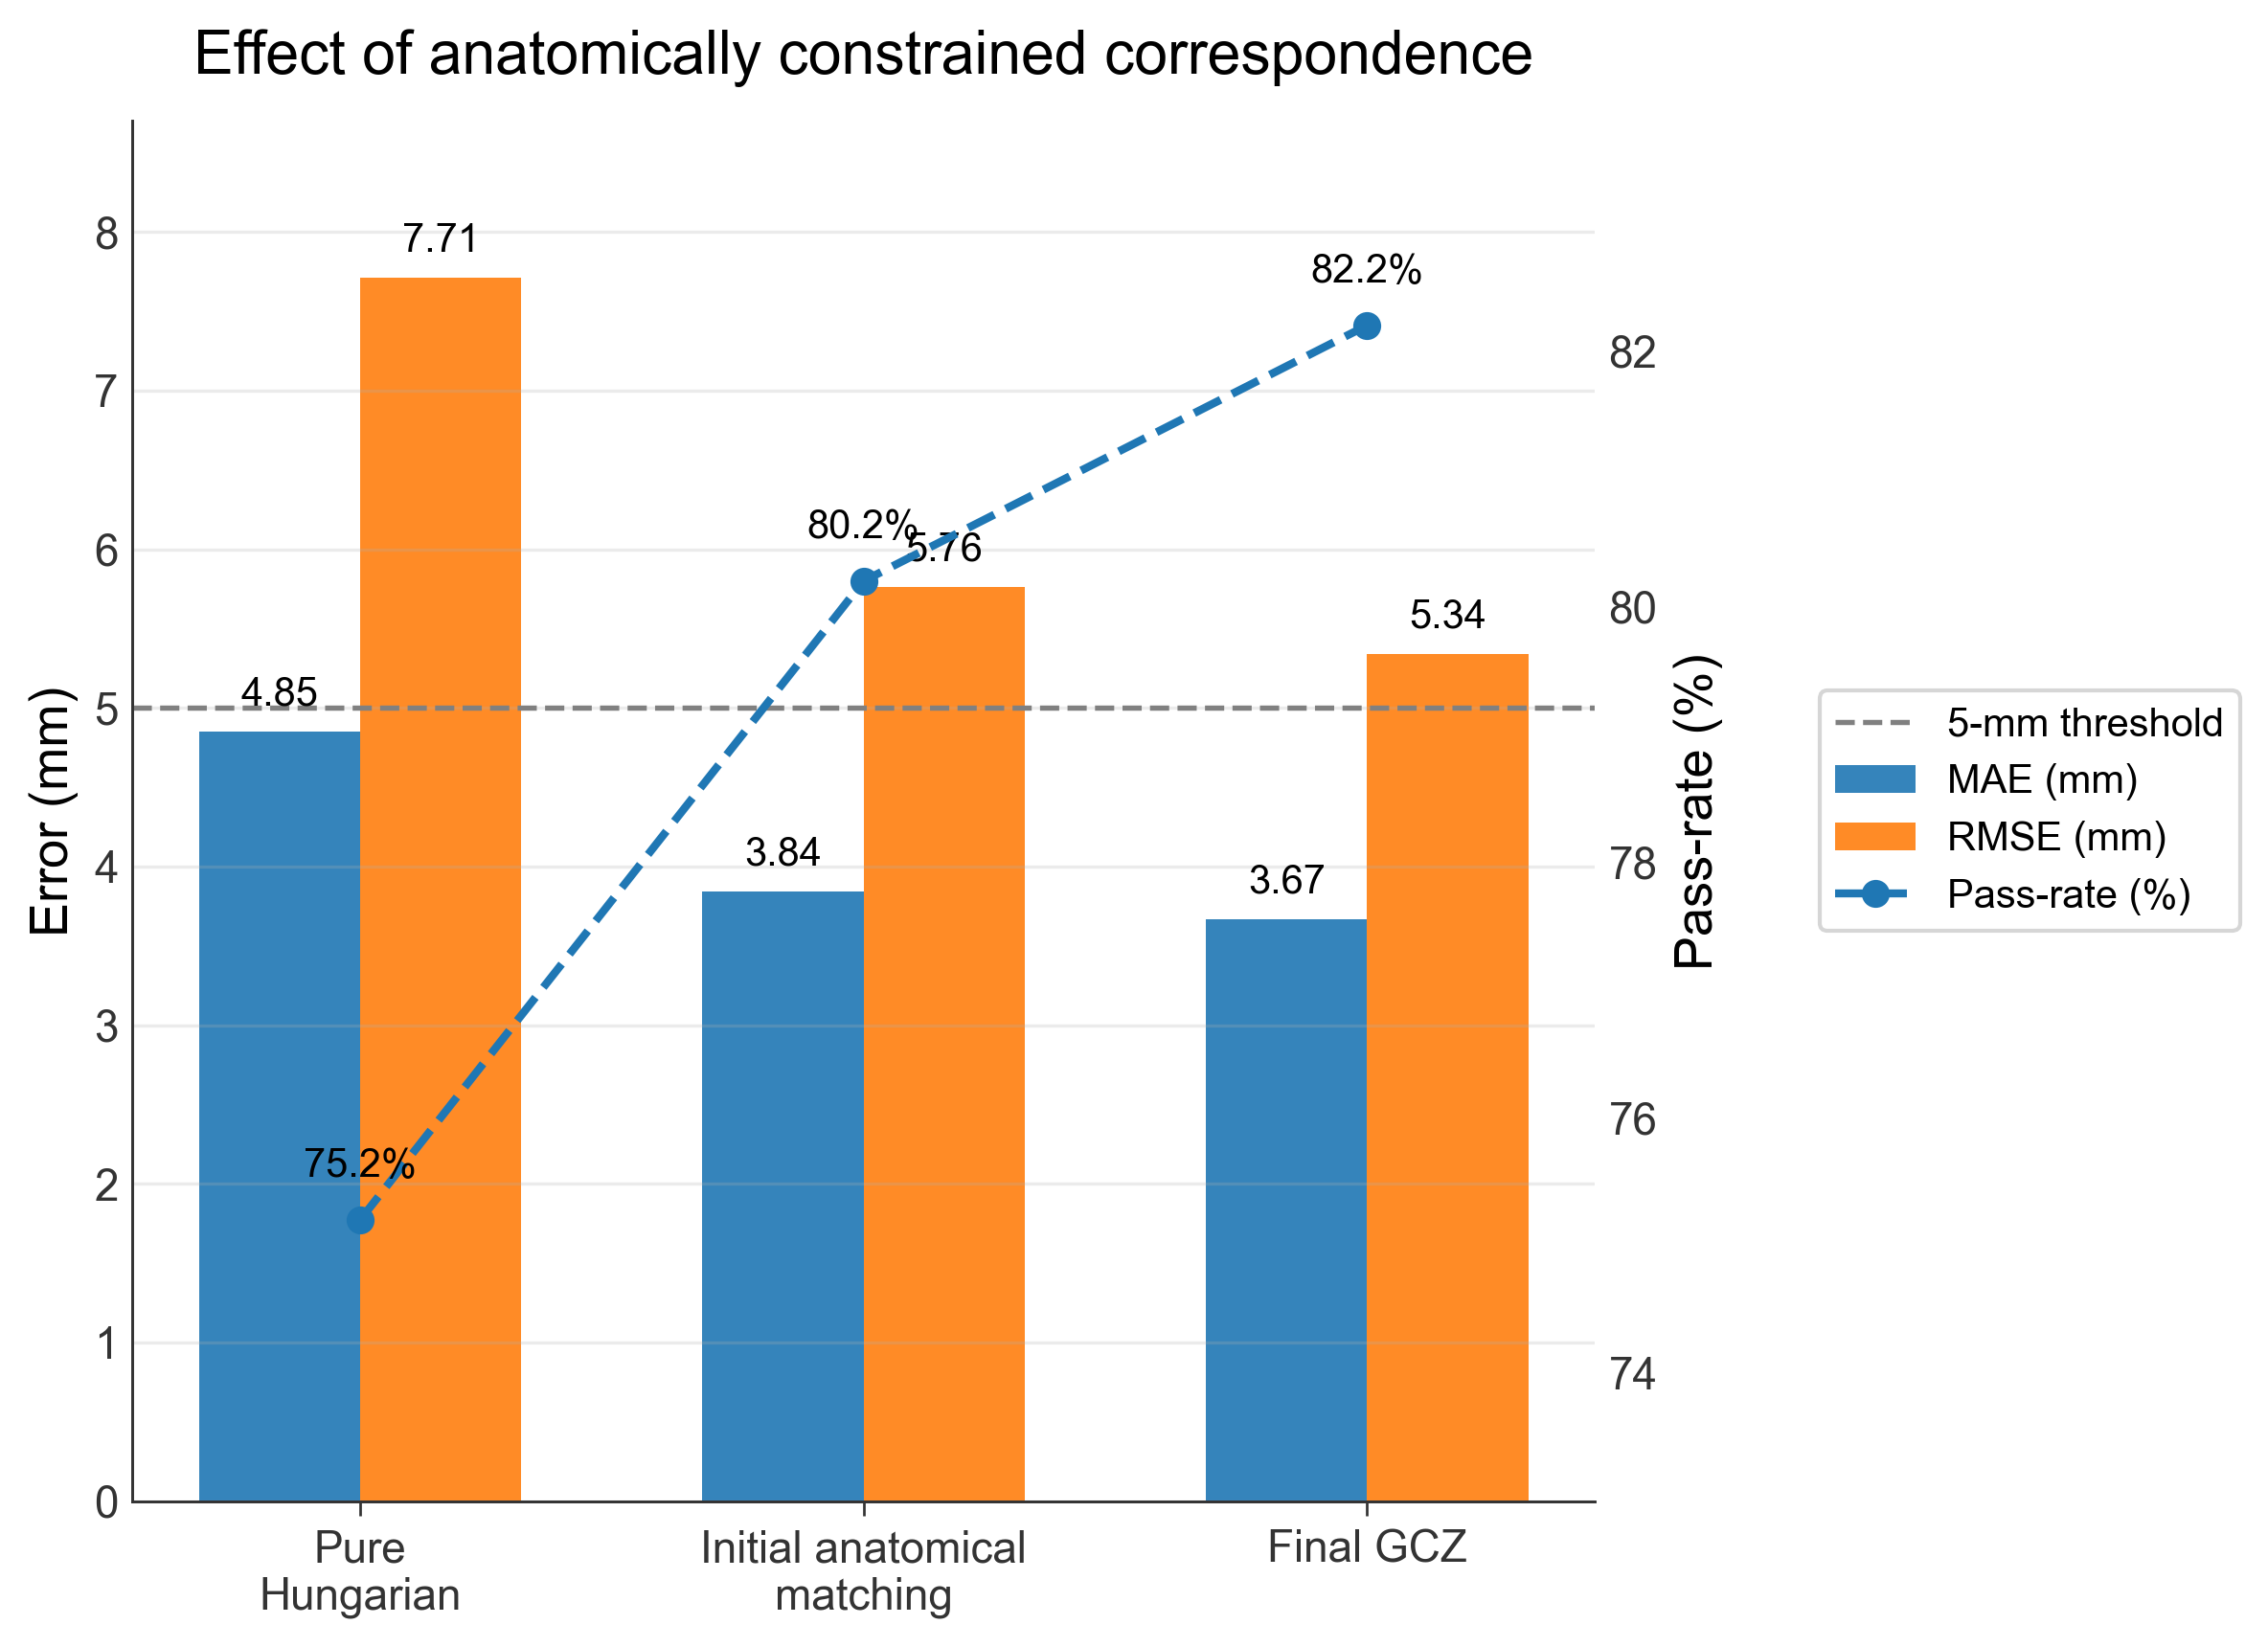
\includegraphics[width=0.62\textwidth]{fig_matching_versions_clean.png}
\caption{Effect of anatomically constrained correspondence on the diagnostic geometry-only GCZ prediction. Bars show pooled MAE and RMSE, and the dashed line shows the percentage of matched pairs within 5~mm (values of Table~\ref{tab:matching_versions}).}
\label{fig:matching_versions}
\end{figure}

\begin{figure}[h]
\centering
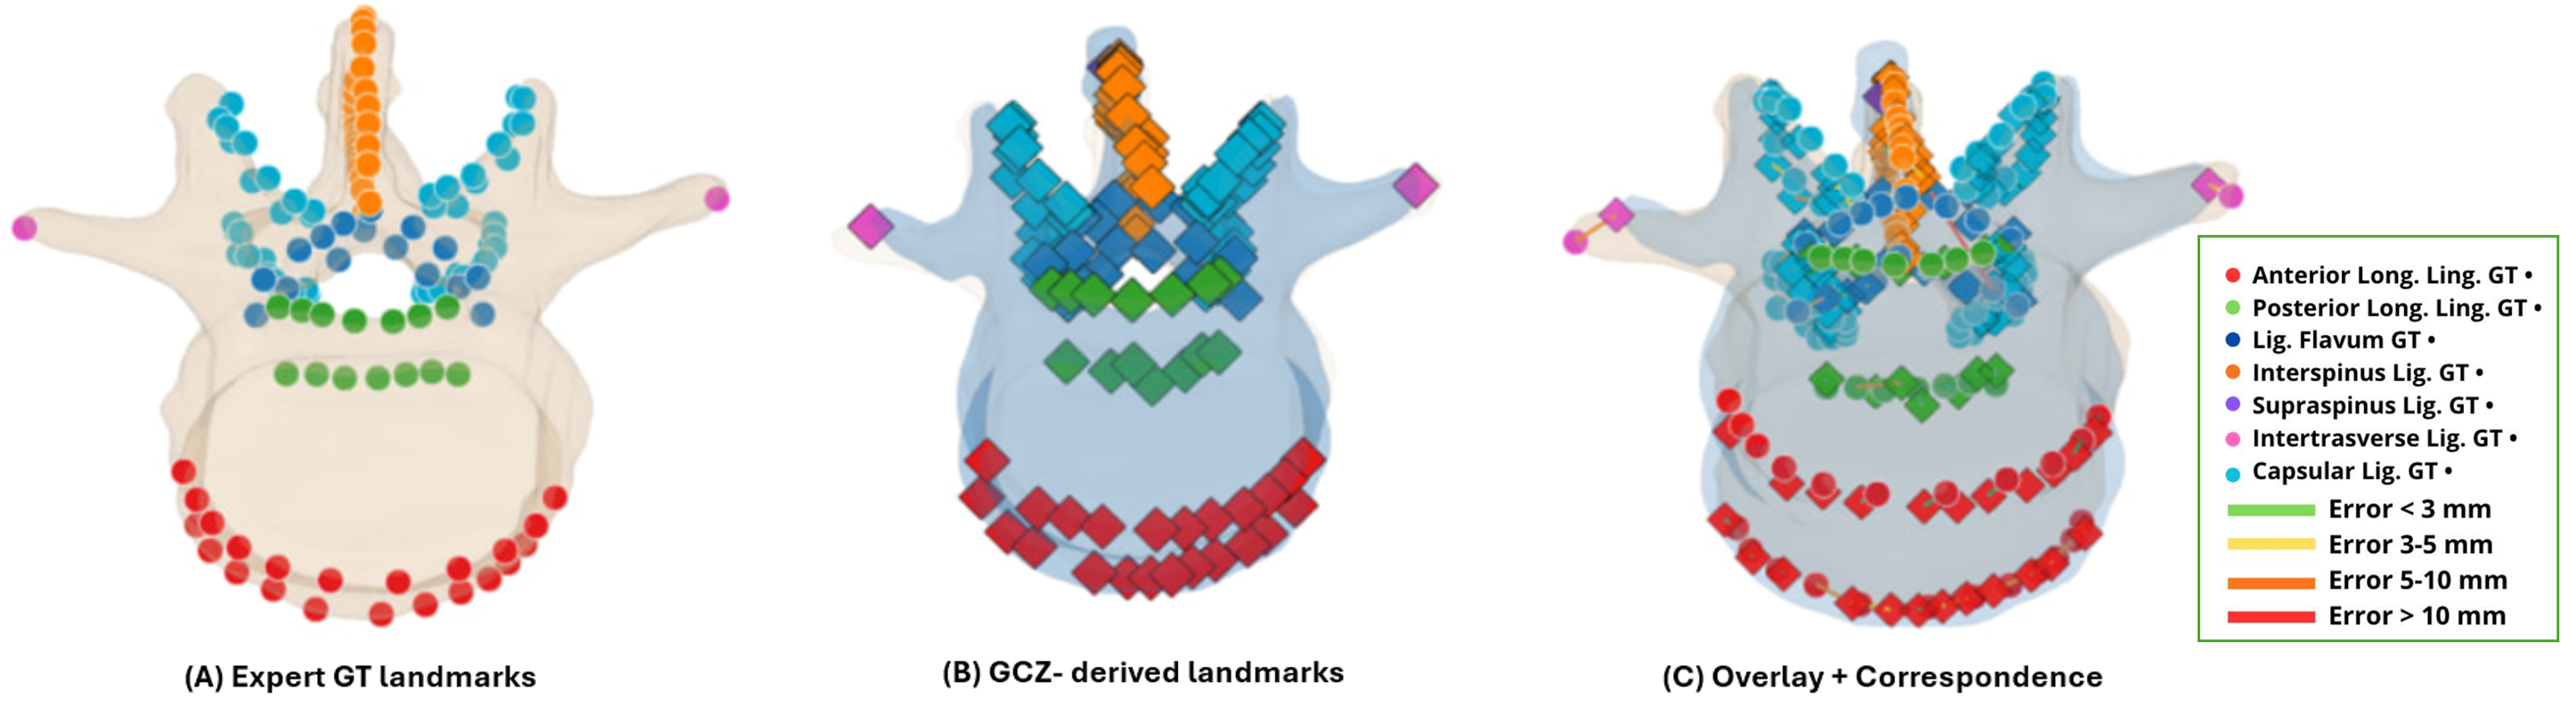
\includegraphics[width=\textwidth]{figure4_cropped_labeled1.png}
\caption{Representative qualitative landmark correspondence on a held-out vertebra of the diagnostic analysis. (A) Expert landmarks. (B) GCZ landmarks transferred from the atlas after alignment. (C) Overlay of expert and GCZ landmarks with correspondence lines; circles indicate expert landmarks and diamonds GCZ landmarks. The overlay exposes side swaps, superior--inferior inversions, and candidate-region failures.}
\label{fig:overlay}
\end{figure}

\section*{S7. Models selected in the primary evaluation}

\begin{table}[h]
\centering
\small
\caption{Extra Trees configuration and blend weight selected for each class by the inner leave-one-subject-out of each outer fold, with the inner validation MAE (mm). $\alpha=0$ keeps the GCZ point.}
\label{tab:selected}
\begin{tabular}{@{}llrlrlr@{}}
\toprule
 & \multicolumn{2}{c}{Held-out S01} & \multicolumn{2}{c}{Held-out S02} & \multicolumn{2}{c}{Held-out S03} \\
\cmidrule(lr){2-3}\cmidrule(lr){4-5}\cmidrule(lr){6-7}
Class & Model, $\alpha$ & MAE & Model, $\alpha$ & MAE & Model, $\alpha$ & MAE \\
\midrule
ALL & ET-4, 0.55 & 3.234 & ET-3, 0.25 & 3.886 & ET-1, 0 & 3.163 \\
PLL & ET-1, 0 & 2.188 & ET-1, 0 & 3.427 & ET-1, 0 & 1.823 \\
LF & ET-1, 0 & 4.482 & ET-1, 0.40 & 1.873 & ET-1, 0 & 2.195 \\
ISL & ET-3, 0.70 & 4.603 & ET-2, 0.70 & 2.325 & ET-4, 0.85 & 2.106 \\
SSL & ET-1, 0.25 & 2.745 & ET-2, 0.40 & 3.309 & ET-1, 0.25 & 3.516 \\
ITL & ET-2, 1.20 & 2.218 & ET-1, 1.20 & 1.694 & ET-4, 1.20 & 1.130 \\
CL & ET-2, 0.25 & 4.780 & ET-1, 0 & 2.882 & ET-1, 1.20 & 2.379 \\
\bottomrule
\end{tabular}
\end{table}

When the inner validation error was identical for several configurations, as for $\alpha=0$, where the configuration does not matter, the first configuration in name order is listed.

\revstart
\section*{S8. Component ablation}

The component analyses decompose the fixed pipeline of the primary evaluation; they were defined after the primary results were known and select nothing. They use the stored ICP geometry and the fold models retrained by \texttt{part2\_patient\_loso\_14/run\_part2.py} with their fixed seeds, and are computed by \texttt{paper/revision\_analyses.py}. For each GCZ point, the residual is predicted by the Extra Trees configuration selected for its class in its fold (Table~\ref{tab:selected}); where $\alpha=0$ was selected, the first configuration in name order (ET-1) supplies the prediction for the intermediate configurations. The complete configuration reproduces the saved GCZ-RL predictions (maximum coordinate difference $6\times10^{-14}$~mm, floating-point rounding). No predicted correction of a held-out point exceeded its bound $\tau_L$, so the raw and bounded residuals coincide. Projecting the GCZ points without a residual changes only ITL, because the GCZ points of the other classes already lie in their projection regions.

The last row of Table~\ref{tab:ablation_class} shows why the side constraint is part of the method. The complete nested procedure of the primary evaluation, including the inner selection of configuration and blend weight, was re-run with the constraint switched off. The inner selection was unchanged except for the ITL blend weight of the S02 fold (1.10 instead of 1.20), and every class except ITL kept its error. For ITL, both points of 2 of the 14 held-out vertebrae were then projected onto the same transverse process, an anatomically invalid configuration that the constraint excludes.

\begin{table}[h]
\centering
\small
\caption{Component ablation of the primary evaluation by ligament class: MAE (mm) over the 14 held-out vertebrae.}
\label{tab:ablation_class}
\resizebox{\textwidth}{!}{%
\begin{tabular}{@{}lrrrrrrr@{}}
\toprule
Configuration & ALL & PLL & LF & ISL & SSL & ITL & CL \\
\midrule
\inputrows{tables/tab_ablation_class.tex}
\bottomrule
\end{tabular}}
\end{table}

Against the strongest geometry-only configuration (GCZ with projection, 2.310~mm), the complete GCZ-RL reduced the macro-averaged MAE to 2.150~mm, and did so for each held-out subject (S01 2.563 to 2.315~mm, S02 2.042 to 1.986~mm, S03 2.273 to 2.117~mm; difference $-0.160$~mm, 95\% interval $-0.234$ to $-0.085$~mm; Wilcoxon $p<0.001$ over the 98 cases, 45 lower, 15 higher, 38 unchanged). The row with $\alpha_L=1$ is a comparison made after the held-out evaluation; it was not used to choose the method, whose blend weights were selected by the nested inner validation. In the complete configuration, 740 of the 742 outputs are vertices of the projection region; the other two (ITL of S01 L5 and S02 L4) keep their GCZ position under the side constraint and are vertices of the GCZ selection region. Over the six classes other than ITL, where projection alone leaves the GCZ points unchanged, it reduced the macro-averaged MAE from 2.316 to 2.209~mm (difference $-0.107$~mm, 95\% vertebra-level cluster-bootstrap interval $-0.175$ to $-0.036$~mm; Wilcoxon $p<0.001$ over 84 vertebra--class cases, 33 lower, 13 higher, 38 unchanged), by 6.4\%, 1.5\%, and 4.6\% for held-out S01, S02, and S03.

\section*{S9. Candidate-region coverage and compactness by held-out subject}

For each held-out vertebra and class, the region used for projection was rebuilt from the training subjects of its fold. Its vertex fraction is the share of mesh vertices inside the region, and its area fraction is the share of the vertebral surface area that belongs to the region, where each vertex carries one third of the area of every incident triangle. Containment is computed as in Section~S4. The GCZ selection step uses the same bands but a wider last fallback (Section~S2); for ITL, which used this fallback in all 14 vertebrae, the selection region covers a median of 40.0\% of the surface, against 0.1\% for the projection region.

\begin{table}[h]
\centering
\small
\caption{Reference landmarks inside the projection region (\%) and median area fraction of the region (\%) by held-out subject.}
\label{tab:compact_subject}
\begin{tabular}{@{}lrrrrrr@{}}
\toprule
 & \multicolumn{2}{c}{Held-out S01} & \multicolumn{2}{c}{Held-out S02} & \multicolumn{2}{c}{Held-out S03} \\
\cmidrule(lr){2-3}\cmidrule(lr){4-5}\cmidrule(lr){6-7}
Class & Inside & Area & Inside & Area & Inside & Area \\
\midrule
\inputrows{tables/tab_compactness_by_subject.tex}
\bottomrule
\end{tabular}
\end{table}

\section*{S10. Residual-learning interpretability}

For every GCZ point of the held-out vertebrae, the true residual is the vector to its Hungarian-paired reference point (Eq.~7 of the main text), and the predicted residual is the output of the selected Extra Trees model before blending. Table~\ref{tab:resid_agree} summarizes their agreement. Table~\ref{tab:importance} reports grouped permutation importance, the increase in the mean Euclidean error of the predicted residual on the held-out vertebrae when the features of one group are permuted jointly across points (30 repetitions per group and fold), and the impurity-based importance of the fitted models summed over the group. Importance describes what the fitted models use; it does not establish an anatomical or causal relation. Figure~\ref{fig:residual_vectors} shows the true and predicted residuals on one held-out vertebra.

\begin{table}[h]
\centering
\small
\caption{Agreement of predicted and true residual vectors on the held-out vertebrae of the primary evaluation (all classes, whether or not the correction was applied). Clipped: after the correction bound. Cosine: cosine of the angle between predicted and true residual. Closer: share of points that the clipped correction alone moves closer to their paired reference point.}
\label{tab:resid_agree}
\begin{tabular}{@{}lrrrrrr@{}}
\toprule
Class & Points & True (mm) & Clipped (mm) & Median cosine & Cosine $>0$ (\%) & Closer (\%) \\
\midrule
\inputrows{tables/tab_residual_agreement.tex}
\bottomrule
\end{tabular}
\end{table}

\begin{table}[h]
\centering
\small
\caption{Grouped feature importance of the residual regressors. Permutation: increase in held-out residual-prediction error, mean and range over the three folds. Impurity: share of the total impurity reduction, averaged over the fitted models of all folds. Groups (feature numbers of Table~\ref{tab:features}): normalized position 1--6 and 32; candidate-region relation 7--19; anatomical context 20--27; local surface geometry 28--31; offset from class prior 33--36.}
\label{tab:importance}
\begin{tabular}{@{}lrrr@{}}
\toprule
Feature group & Permutation (mm) & Range over folds & Impurity share \\
\midrule
\inputrows{tables/tab_importance.tex}
\bottomrule
\end{tabular}
\end{table}

By impurity, the ten most used single features were the position of the point in the calibrated $y_n$ band (feature 9; 0.119), the superior--inferior and lateral components of the direction to the class prior (features 35 and 34; 0.080 and 0.057), the normalized lateral position (feature 1; 0.059), the signed lateral position (feature 32; 0.057), the distance to the region box boundary (feature 8; 0.051), the vertebral level (feature 20; 0.034), the distance from the mid-sagittal plane (feature 4; 0.034), and the normalized superior--inferior position and its repeat (features 3 and 6; 0.033 each). Grouped permutation importance ranked the groups differently in each fold (anatomical context first for held-out S01, normalized position for S02, local surface geometry for S03), so no single group dominates.

\begin{figure}[h]
\centering
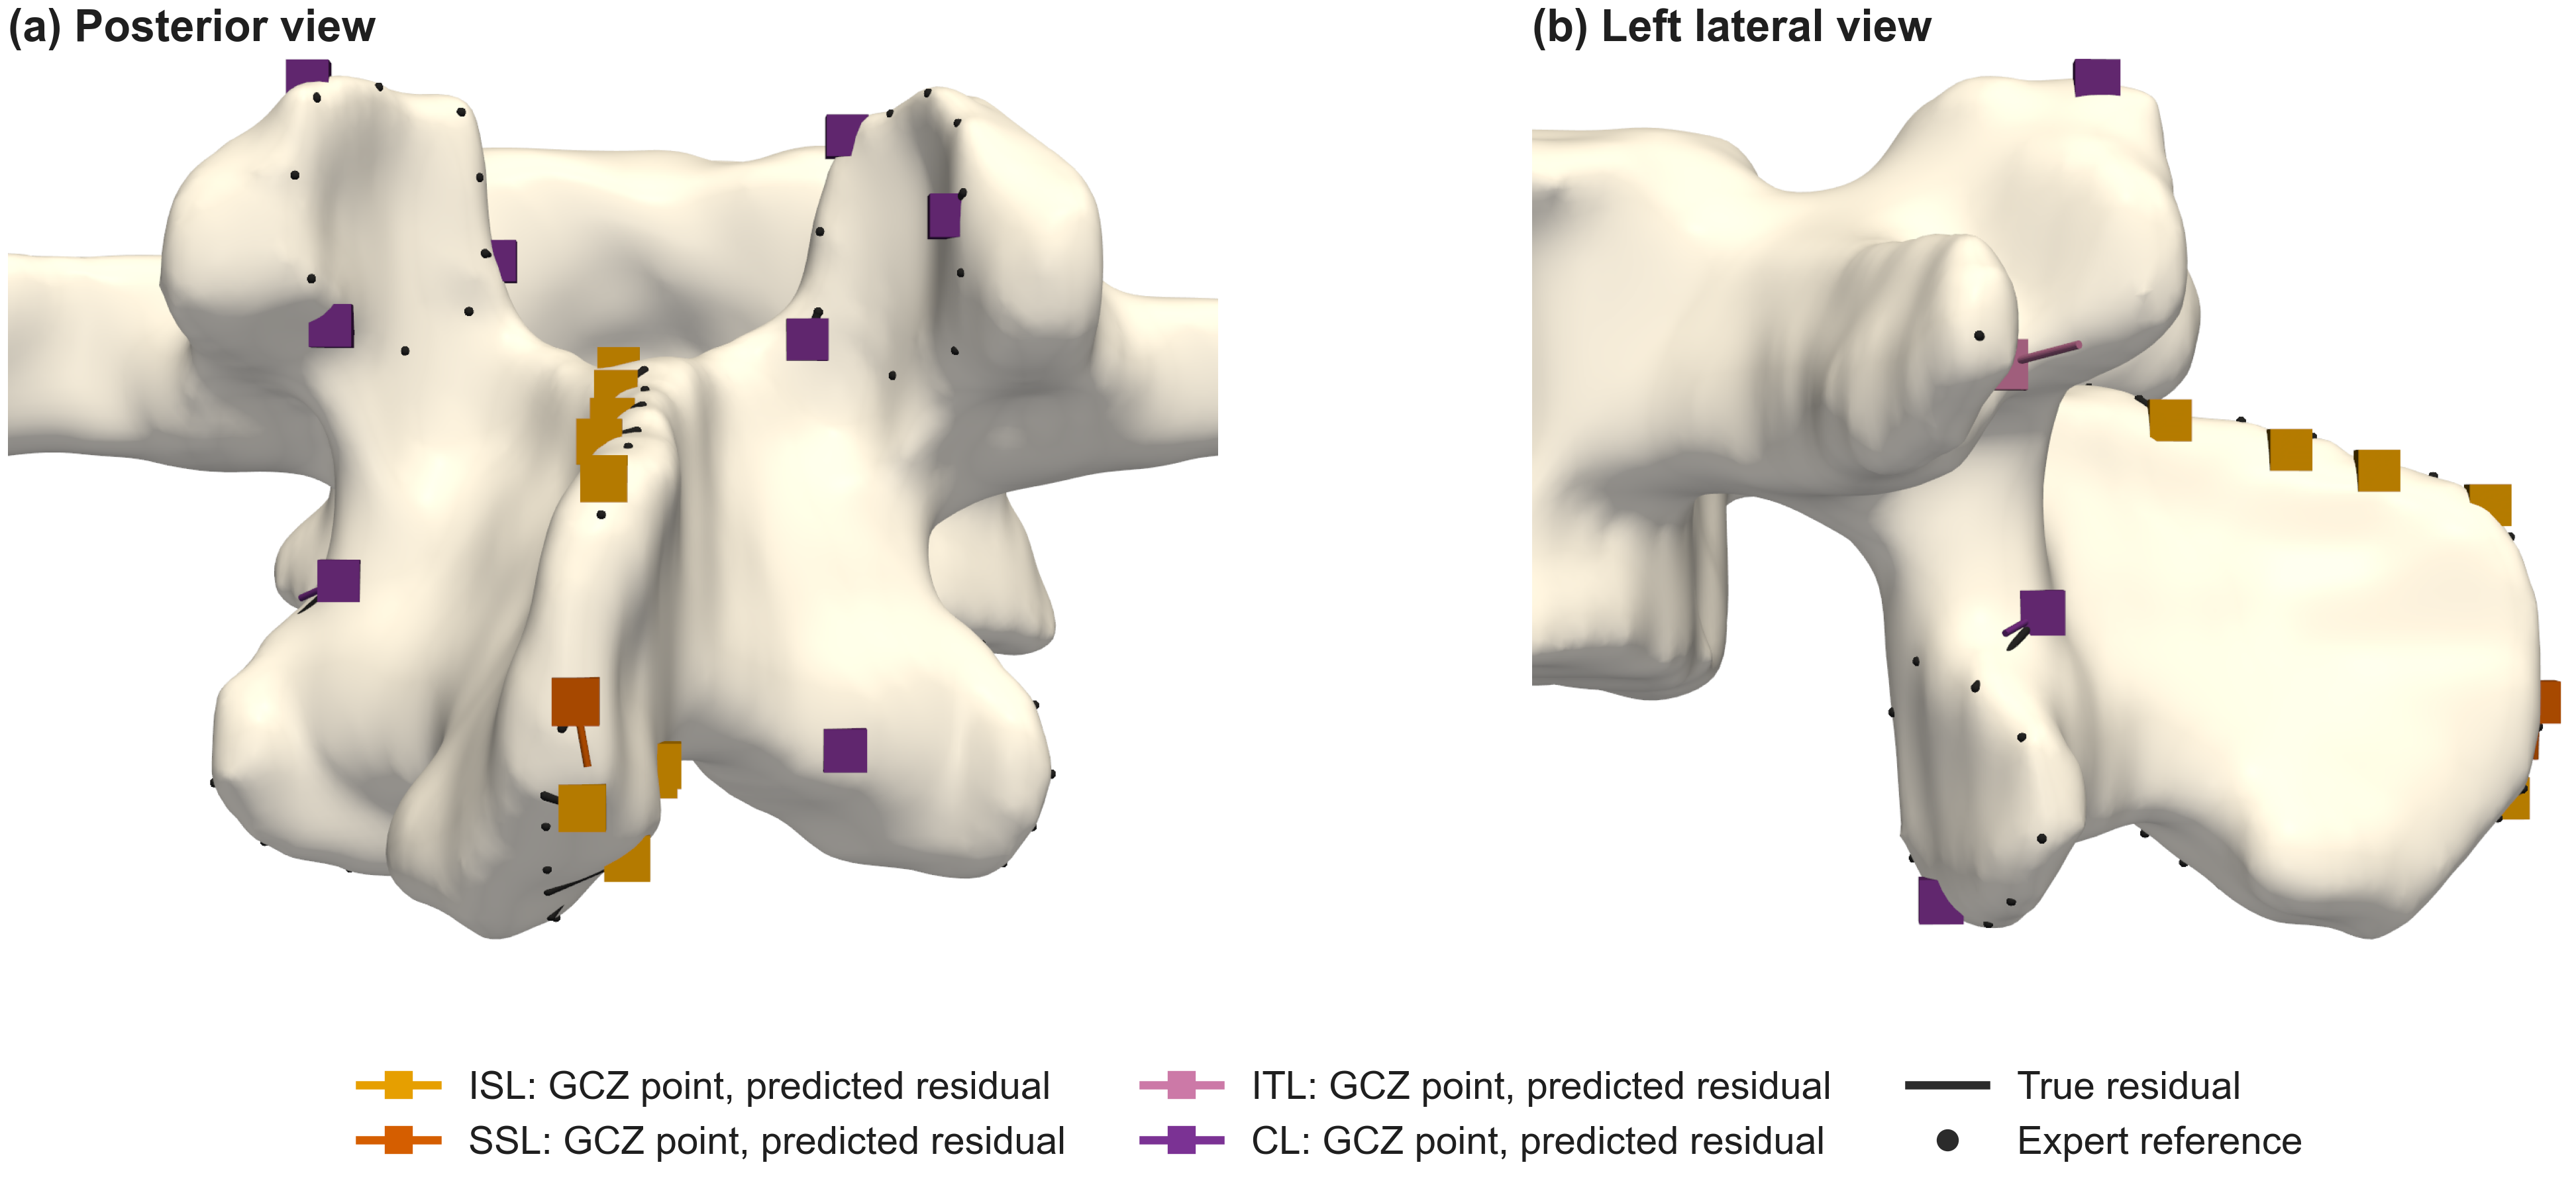
\includegraphics[width=\textwidth]{figS3_residual_vectors.png}
\caption{True (dark) and predicted (colored) residual vectors of the GCZ points (colored squares) on held-out vertebra S03 L4 (lumbar level L4; fold holding out S03), for the classes whose correction was applied in this fold (blend weight above zero): ISL, SSL, ITL, and CL. Small dark points are the expert reference landmarks of these classes. Vectors are drawn at true length, before the correction bound and projection. The applied corrections are shown in Fig.~\ref{fig:correction_real}.}
\label{fig:residual_vectors}
\end{figure}

\section*{S11. Atlas selection and registration sensitivity}

Table~\ref{tab:atlas} lists, for each held-out vertebra of the primary evaluation, the atlas vertebra selected with the stored ICP alignments, whether it is of the same level, its quick-ICP residual, and the per-vertebra macro-averaged MAE of GCZ and GCZ-RL, together with the same quantities from the second computing environment (Section~S5). The second environment is a recomputation on the same data, not an independent cohort. Same-level atlases were selected for 7 vertebrae and cross-level atlases for 7; mean per-vertebra GCZ errors were 3.073 and 2.686~mm, and mean GCZ-RL errors 2.203 and 2.098~mm. The quick-ICP residual was not associated with the per-vertebra error (Spearman $\rho=0.24$, $p=0.40$ for GCZ; $\rho=0.25$, $p=0.38$ for GCZ-RL). No new perturbation of the registration was performed for this analysis.

\begin{table}[h]
\centering
\small
\caption{Atlas selection and per-vertebra error (mm) of the primary evaluation, with the stored ICP alignments and with the alignments recomputed in a second computing environment. $^{*}$Atlas changed.}
\label{tab:atlas}
\resizebox{\textwidth}{!}{%
\begin{tabular}{@{}lllrrrlrrr@{}}
\toprule
 & \multicolumn{5}{c}{Stored alignments (reported results)} & \multicolumn{4}{c}{Second environment} \\
\cmidrule(lr){2-6}\cmidrule(lr){7-10}
Target & Atlas & Level & Residual & GCZ & GCZ-RL & Atlas & Residual & GCZ & GCZ-RL \\
\midrule
\inputrows{tables/tab_atlas.tex}
\bottomrule
\end{tabular}}
\end{table}

\FloatBarrier
\section*{S12. Reproducibility verification}

Table~\ref{tab:repro} compares the main reported values with the values regenerated from the public data by the code release (\texttt{paper/reproducibility\_check.py}). Level A: metrics recomputed from the saved predictions and the annotations. Level B: end-to-end re-run with the stored ICP alignments and SLD output, with every Extra Trees model retrained with its fixed seed. Level C: ICP geometry recomputed from scratch; the leakage test was re-executed in this way, whereas the second-environment values of Section~S5 are archived outputs that were not re-executed. The leakage test with recomputed ICP compared 412 points instead of 424, because the recomputed alignment selected a different atlas for S02 L3 (Section~S11), and again found no difference. The S02 reduction of the submitted draft (10.1\%) had been computed from rounded subject means; the unrounded value is 10.0\%.

{\footnotesize
\begin{longtable}{@{}P{42mm}rrrP{12mm}P{36mm}P{22mm}@{}}
\caption{Reproducibility verification of the main reported values.}\label{tab:repro}\\
\toprule
Claim & Reported & Reproduced & $|\Delta|$ & Level & Source file & Status \\
\midrule
\endfirsthead
\toprule
Claim & Reported & Reproduced & $|\Delta|$ & Level & Source file & Status \\
\midrule
\endhead
\inputrows{tables/reproducibility_table.tex}
\bottomrule
\end{longtable}}

\section*{S13. Sensitivity to the ICP seeds}

The atlas selection and alignment of GCZ use random point samples in ICP (Section~S5). To quantify how much the results depend on this step, the complete nested procedure of the primary evaluation was re-run ten times with the ICP geometry recomputed from scratch, with every random seed of the ICP point sampling (quick ICP of each candidate atlas, residual sample, full alignment) shifted by a fixed offset per run (\texttt{paper/icp\_seed\_sensitivity.py}). Everything else was unchanged: the three LOSO folds and their subjects, the calibrated regions (computed from annotations only), the fallback template and farthest-point sampling seeds, the Extra Trees configurations and seeds, the model and blend-weight grids, the nested inner selection, and the evaluation. The residual training data change only as a consequence of ICP, because the training-side GCZ predictions are also recomputed. The stored checkpoints were neither read nor written. Offset~0 uses the seeds of the method and reproduces the second-environment run of Section~S5 exactly (GCZ 3.208, GCZ-RL 2.418~mm). The ten runs are a computational sensitivity analysis on the same three subjects, not additional subjects or an external validation.

Across the ten runs, 2--4 of the 14 held-out vertebrae changed atlas relative to the stored alignments, most often at L3 (S02 L3 in 8 runs). GCZ-RL improved on GCZ in every run, by 22.8--33.4\% (mean 26.9\%), and for every held-out subject in every run (30 of 30 comparisons). Its macro-averaged MAE ranged from 2.103 to 2.918~mm (mean $2.357\pm0.239$~mm), against 2.844 to 3.888~mm for GCZ (mean $3.226\pm0.309$~mm). SLD, which does not use ICP, is 2.224~mm in every run; GCZ-RL was below it in 3 of the 10 runs. The reported results (stored alignments: 2.150 and 2.879~mm) lie in the lower part of these ranges.

\begin{table}[h]
\centering
\small
\caption{Primary evaluation with the ICP alignments recomputed for ten seed offsets. MAE in mm (macro average over classes); reduction of GCZ-RL relative to GCZ; Pass@5 of GCZ-RL (\%, averaged over vertebra--class cases); GCZ-RL MAE by held-out subject; held-out subjects improved by GCZ-RL over GCZ; held-out vertebrae whose atlas differs from the stored alignments.}
\label{tab:icp_seeds}
\resizebox{\textwidth}{!}{%
\begin{tabular}{@{}lrrrrrrrrr@{}}
\toprule
Offset & GCZ & GCZ-RL & Reduction (\%) & Pass@5 & S01 & S02 & S03 & Subjects improved & Atlas changed \\
\midrule
\inputrows{tables/tab_icp_seeds.tex}
\bottomrule
\end{tabular}}
\end{table}

The ten-seed figure of Section~4.4 of the main text plots these runs together with the reported run.

\section*{S14. Anatomical verification of the candidate regions}

The candidate regions of the primary evaluation were compared with the expert annotations of the same class on all 14 held-out vertebrae (\texttt{paper/region\_verification.py}). The regions were rebuilt exactly as in the method from the training subjects of each fold; nothing was shrunk, moved, or redrawn, and the rendering in the main text colours exactly the vertices of each region mask. The footprint of a class is taken as the mesh surface within 2.5~mm of its expert points. Table~\ref{tab:region_verification} gives, per class, the calibrated bands of the fold holding out S03 and the medians over the 14 vertebrae.

The broad regions of ALL, PLL, and CL follow from the calibration: the superior and inferior parts of these classes (and, for CL, the left and right parts) are pooled into one band per quantity, and their normalized heights vary between training vertebrae, so the $z_n$ band covers both parts and the surface between them, for example the anterior body surface and the anterior parts of both endplates for ALL (Section~S16). The LF region overlaps the CL and PLL regions by most of its area, so the class of a landmark is determined by the transferred atlas landmark rather than by the region. The ITL band of $|x_n-0.5|$ collapses to the most lateral vertices, so the ITL region is narrower than the annotated tip footprint and contains 30\% of its area, although 92.9\% of the ITL points have their nearest vertex inside it. All GCZ-RL landmarks are vertices of the projection region of their class except the two ITL points that keep their GCZ position under the side-preserving fallback (Section~3.10). Tighter regions for the classes with superior and inferior parts would require a body-relative height coordinate (Section~S16); this would be a change of the method and is left for future work.

\begin{table}[h]
\centering
\small
\caption{Candidate regions against expert footprints on the 14 held-out vertebrae (medians; Inside pooled over reference points). Bands: calibrated $\mu_L\pm2\sigma_L$ bands in the fold holding out S03. Area: share of the vertebral surface. Footprint: surface within 2.5~mm of an expert point of the class. Ratio: region area over footprint area. Foot.\ in reg.: share of the footprint area inside the region. Reg.\ on foot.: share of the region area within the footprint. Overlap: share of the region area that also belongs to another class region.}
\label{tab:region_verification}
\resizebox{\textwidth}{!}{%
\begin{tabular}{@{}llllrrrrrrr@{}}
\toprule
Class & $y_n$ band & $|x_n-0.5|$ band & $z_n$ band & Inside (\%) & Region area (\%) & Footprint area (\%) & Ratio & Foot.\ in reg.\ (\%) & Reg.\ on foot.\ (\%) & Overlap (\%) \\
\midrule
\inputrows{tables/tab_region_verification.tex}
\bottomrule
\end{tabular}}
\end{table}

\section*{S15. Method illustrations on real data}

Figures~\ref{fig:pipeline_real} and~\ref{fig:correction_real} show the steps of Fig.~1 and the correction of Fig.~5 of the main text on held-out vertebra S03 L4 of the primary evaluation, using the real meshes and the saved landmarks (\texttt{paper/figures\_main.py}). The ICP transfer in Fig.~\ref{fig:pipeline_real}(c) is recomputed with the seed of the primary run and reproduces the saved GCZ landmarks of this vertebra (maximum deviation $6\times10^{-14}$~mm).

\begin{figure}[h]
\centering
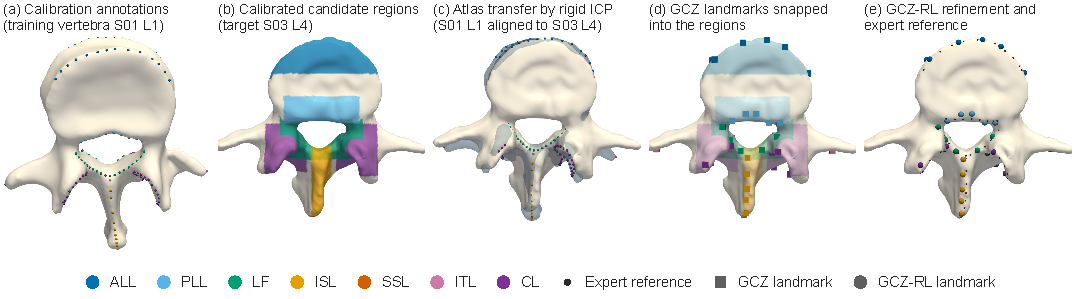
\includegraphics[width=\textwidth]{fig1_pipeline.pdf}
\caption{GCZ-RL on held-out vertebra S03 L4 (fold holding out S03), superior view. (a) Expert annotations of a training vertebra (S01 L1, the atlas selected for this target). (b) Candidate regions of the target, calibrated on S01 and S02. (c) The atlas aligned to the target by rigid ICP and its transferred landmarks. (d) GCZ landmarks snapped to target vertices inside the regions. (e) GCZ-RL landmarks after the bounded residual correction and projection, with the expert reference; dark segments connect each GCZ landmark to its corrected position.}
\label{fig:pipeline_real}
\end{figure}

\begin{figure}[h]
\centering
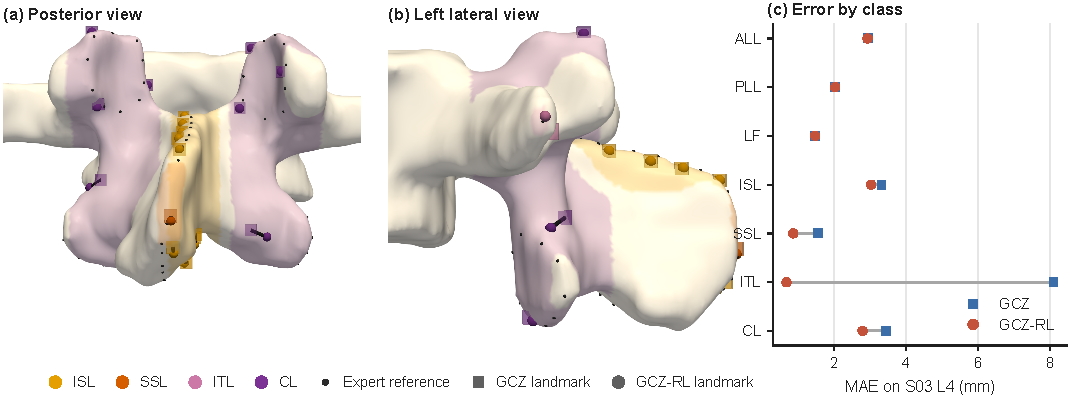
\includegraphics[width=\textwidth]{fig4_residual_correction.pdf}
\caption{Applied correction on held-out vertebra S03 L4 for the classes whose blend weight was above zero in this fold (ISL, SSL, ITL, CL). (a, b) Translucent squares: GCZ landmarks; spheres: GCZ-RL landmarks after the bounded correction and projection onto the tinted candidate region; dark segments: the applied correction; small dark points: expert reference. (c) MAE of each class on this vertebra before (GCZ) and after (GCZ-RL); for ALL, PLL, and LF the inner validation selected $\alpha_L=0$, so the two coincide.}
\label{fig:correction_real}
\end{figure}

\FloatBarrier
\section*{S16. Superior and inferior margins of ALL and PLL}

The ALL and PLL annotations are stored as superior and inferior parts along the margins of the vertebral body. On the 14 held-out vertebrae, \texttt{paper/margin\_verification.py} checks the orientation and normalization of the coordinates and the position of the regions and landmarks relative to these margins (Fig.~\ref{fig:margins}); nothing is changed.

\emph{Orientation and normalization.} In the frame of the meshes ($+z$ superior), the superior part lies above the inferior part in all 28 vertebra--class cases, by a median of 27.5~mm for ALL and 27.4~mm for PLL (minimum 24.4~mm). On S03 L4, the body margins measured on the mesh alone agree with the expert parts within 1.6~mm. The normalized height $z_n$ used by the method equals $(z-z_{\min})/(z_{\max}-z_{\min})$ over the whole vertebra.

\emph{Regions.} The margins of the vertebral body lie at different normalized heights in different vertebrae, because $z_n$ is measured over the whole vertebra, including the posterior elements: the inferior ALL margin lies between $z_n=0.05$ and $0.50$ and the superior between $0.50$ and $0.97$ (Fig.~\ref{fig:margins}d,e). A band that contains the margins of all training vertebrae spans 0.00--1.00 for ALL and 0.04--1.00 for PLL in the fold holding out S03, so the ALL and PLL regions cover the anterior and posterior body walls over their full height together with the adjacent rim of the endplates (Fig.~\ref{fig:margins}a--c). A median of 28\% (ALL) and 35\% (PLL) of the region area lies in the middle half between the two margins.

\emph{Landmarks.} The superior--inferior position of the landmarks is set by the atlas transfer, which carries the margins of the atlas vertebra to the target, and the region constrains their antero-posterior and lateral position. None of the 140 ALL and 140 PLL landmarks of GCZ, and none of GCZ-RL, lies in the middle half between the margins: all lie at the superior or inferior margin, as do the expert points.

\emph{Separate bands.} Calibrating separate bands for the superior and inferior parts would not tighten the ALL region (the two bands together span 0.00--1.00 in the folds holding out S02 and S03) and would remove about 45\% of the PLL region, but 8 ALL and 18 PLL landmarks of GCZ-RL, all at the margins of their vertebrae, would fall outside these bands, because the margin heights of some held-out vertebrae lie beyond the range of the training vertebrae. Tighter regions for these classes would therefore require a body-relative height coordinate rather than separate bands.

\begin{figure}[h]
\centering
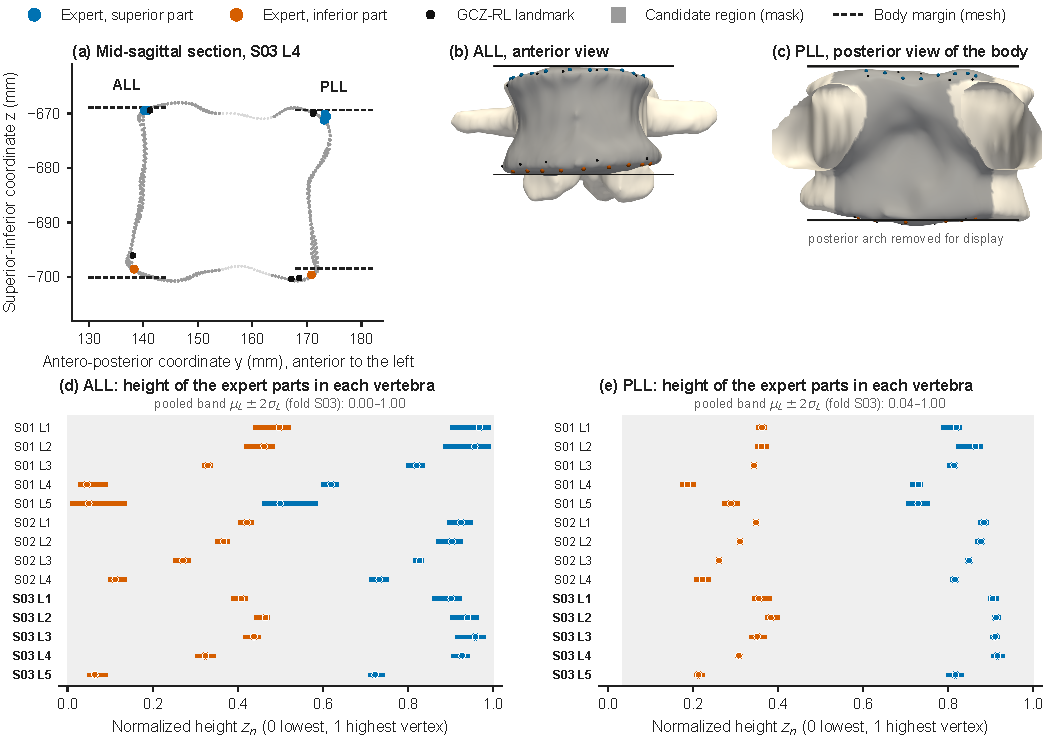
\includegraphics[width=\textwidth]{fig_margins_ALL_PLL.pdf}
\caption{Superior and inferior margins of ALL and PLL. (a) Mid-sagittal section of held-out vertebra S03 L4 in millimeters (anterior to the left, superior up): mesh vertices within 1.5~mm of the mid-sagittal plane (light), vertices of the ALL and PLL candidate regions (gray), body margins measured on the mesh (dashed), and the expert points and GCZ-RL landmarks within 6~mm of the plane. (b) ALL region, anterior view. (c) PLL region, posterior view of the vertebral body with the posterior arch removed for display. Solid lines in (b, c): body margins measured on the mesh. Regions calibrated on S01 and S02, as in the method. (d, e) Normalized height $z_n$ of the superior and inferior expert parts in each of the 14 vertebrae (dot: mean; bar: range; held-out subject S03 in bold) and the pooled band of the fold holding out S03 (shaded).}
\label{fig:margins}
\end{figure}

\FloatBarrier
\section*{S17. Complete qualitative comparison of the three methods}

Figure~\ref{fig:qualitative_complete} is the qualitative figure of the previous version of the manuscript, unchanged. It shows the predictions of GCZ, GCZ-RL, and SLD for all seven classes on held-out vertebra S03 L4 in three orthogonal views (\texttt{paper/fig6\_qualitative\_loso.py}). The main text shows the same vertebra with magnified close-ups of the classes whose correction is active in this fold (Fig.~7) and the expert annotations, search regions, and GCZ-RL landmarks class by class (Fig.~8).

\begin{figure}[h]
\centering
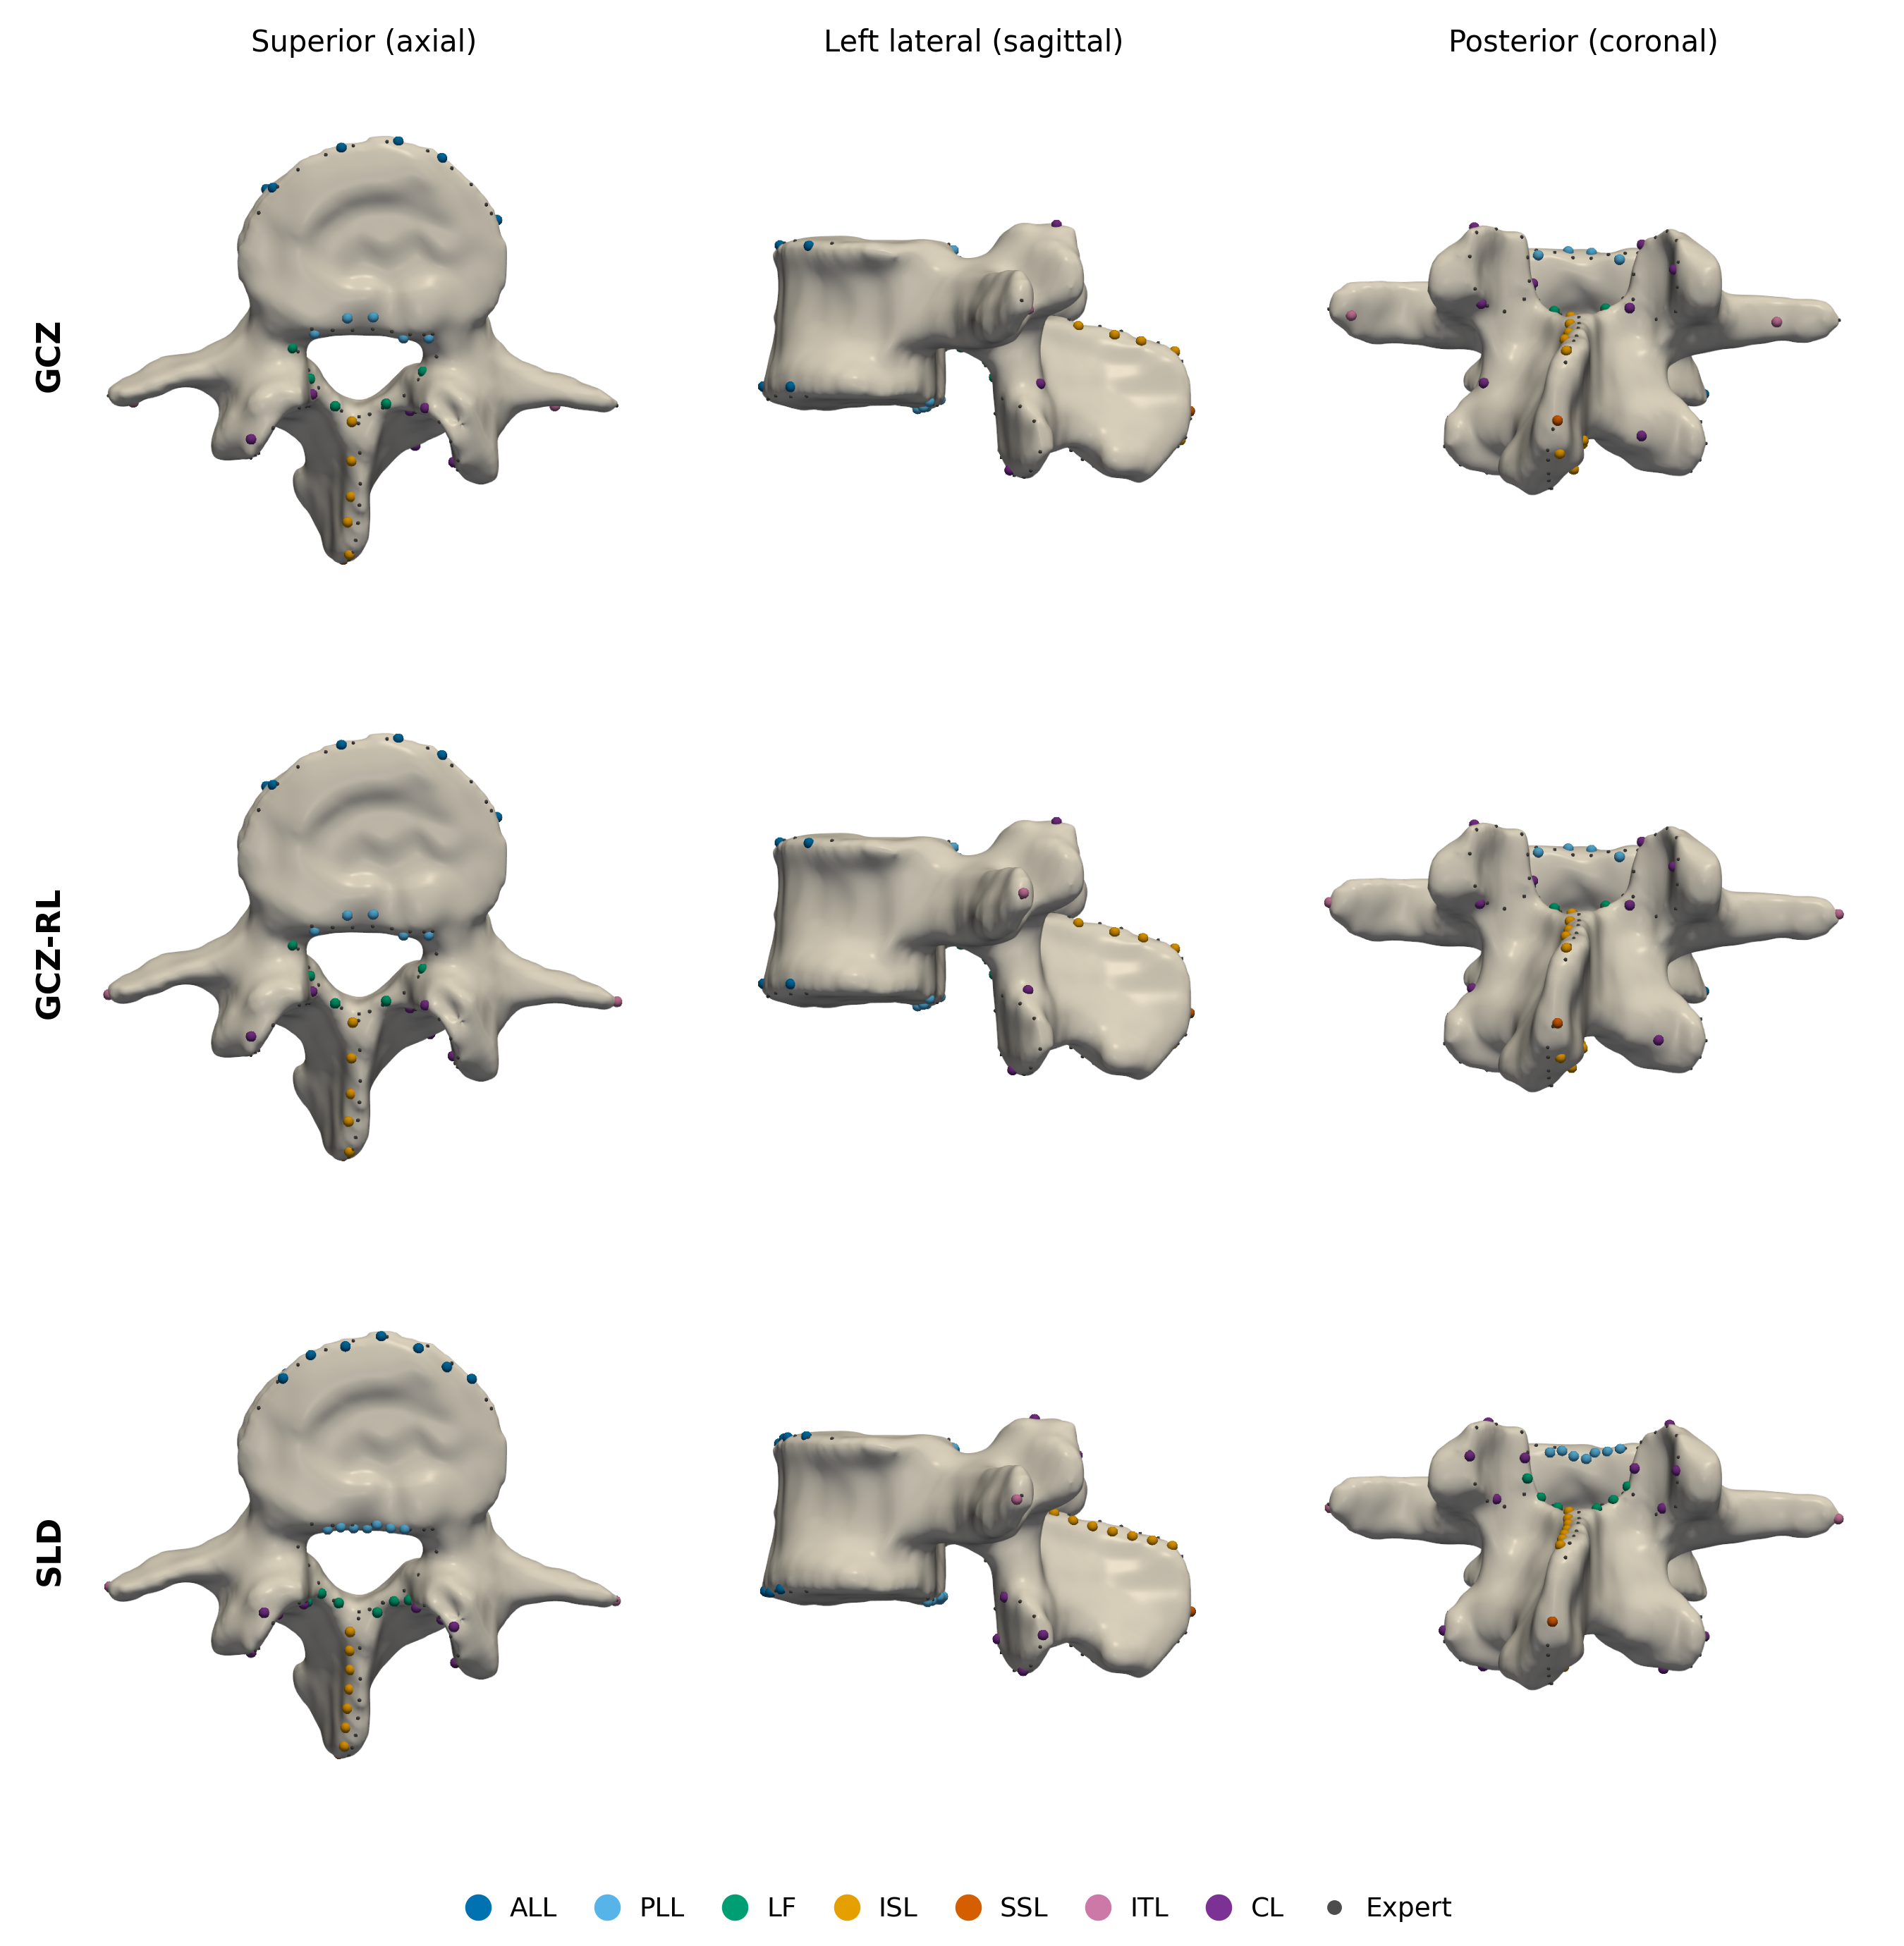
\includegraphics[width=0.82\textwidth]{fig_qualitative_loso_S03_L4.png}
\caption{Predictions of GCZ, GCZ-RL, and SLD on held-out vertebra S03 L4 of the primary evaluation (fold holding out S03), shown in three orthogonal views. Small dark points are the expert reference landmarks; colored spheres are the predicted landmarks of each class. ITL improves from 8.09 to 0.68~mm, and CL, ISL, and SSL also change, whereas for ALL, PLL, and LF the inner validation of this fold selected $\alpha=0$, so GCZ and GCZ-RL coincide. Macro-averaged errors on this vertebra are 3.263~mm for GCZ, 1.972~mm for GCZ-RL, and 2.771~mm for SLD. All points are read from the saved predictions of the code release.}
\label{fig:qualitative_complete}
\end{figure}

\FloatBarrier
\section*{S18. Calibrated GCZ search regions}

Figure~\ref{fig:search_regions} shows the calibrated GCZ search regions of held-out vertebra S03 L4, the masks used for projection in the primary evaluation, exactly as computed by \texttt{gcz.candidate\_vertices} from the training subjects S01 and S02, together with the expert annotations (\texttt{paper/figures\_anatomy.py}). They are search regions, not attachment footprints: for ALL, PLL, and CL they also cover the surface between the superior and inferior attachment margins, because one band must contain the margins of all training vertebrae (Section~S16). The attachment footprints and the GCZ-RL landmarks, which lie on the margins, are shown in Fig.~8 of the main text.

\begin{figure}[h]
\centering
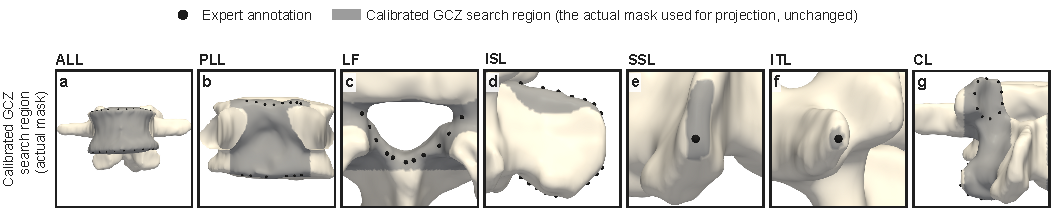
\includegraphics[width=\textwidth]{fig_search_regions.pdf}
\caption{Calibrated GCZ search regions (gray; the actual masks used for projection, unchanged) and expert annotations (black) on held-out vertebra S03 L4 for (a) ALL, anterior view; (b) PLL, posterior view of the vertebral body with the posterior arch removed for display; (c) LF, superior view; (d) ISL, left lateral view; (e) SSL, posterior view of the spinous process tip; (f) ITL, lateral view of the left transverse process tip; (g) CL, posterior view of the left side. Every gray vertex belongs to the region mask of the method. The cameras and crops are those of Fig.~8(g--k).}
\label{fig:search_regions}
\end{figure}

\FloatBarrier
\section*{S19. Step-by-step correction of the ITL landmarks of S03 L4}

The ITL error of held-out vertebra S03 L4 falls from 8.095~mm (GCZ) to 0.678~mm (GCZ-RL), the largest change in Fig.~7 of the main text. Table~\ref{tab:itl_trace} follows both ITL landmarks through every operation of the correction (\texttt{paper/itl\_trace.py}): the saved Extra Trees model of the fold holding out S03 predicts a residual, which is clipped to the correction radius, added to the GCZ landmark, and projected onto the calibrated ITL region; the result is blended with the GCZ landmark by the weight $\alpha_L$ selected in the inner validation and projected again, with each landmark kept on its side. The computation uses only the target mesh, the saved GCZ landmarks, and the saved fold model with its thresholds, class priors, correction radius, and $\alpha_L$, all derived from S01 and S02; the expert annotations of S03 are read only afterwards, to score each step. It reproduces the saved GCZ-RL landmarks exactly (maximum deviation 0~mm), and the scored class errors equal those of the evaluation. Each landmark is scored against the reference of its own side (Hungarian matching pairs the right landmark with the right tip and the left with the left).

The two GCZ landmarks lie on the transverse processes, inside the wide GCZ selection region and outside the small projection region at the tips. Without projection, the learned residual moved the right landmark 8.48~mm towards the tip (error 11.51 to 6.71~mm) and left the left landmark at its error (4.68 to 4.73~mm); clipping was not active (radius 15.98~mm). Projecting the GCZ landmarks onto the ITL region without any residual already reduces the class error to 1.133~mm, and the complete correction to 0.678~mm. Most of the ITL improvement on this vertebra therefore comes from the projection onto the calibrated region, which is part of the GCZ-RL framework, and the learned residual adds 0.455~mm; it is not an improvement of the Extra Trees regressor alone. This agrees with the component analysis of the main text, in which projection alone accounts for most of the ITL change over the cohort.

\begin{table}[h]
\centering
\small
\caption{Step-by-step GCZ-RL correction of the two ITL landmarks of held-out vertebra S03 L4 (fold holding out S03; Extra Trees configuration ET-4, $\alpha_L=1.2$). Step: length of the displacement from the previous step (for the last row, from the GCZ landmark). Error: distance to the expert reference of the same side. Region: whether the point is a vertex of the calibrated ITL projection region. The last row of each side is the counterfactual projection of the GCZ landmark without residual.}
\label{tab:itl_trace}
\begin{tabular}{@{}llrrl@{}}
\toprule
Side & Operation & Step (mm) & Error (mm) & Region \\
\midrule
\inputrows{tables/tab_itl_trace.tex}
\bottomrule
\end{tabular}
\end{table}
\revend

\FloatBarrier
\begin{thebibliography}{1}
\bibitem[Blomenkamp et al.(2026)]{blomenkamp2026sld}
Blomenkamp, L., Kramer, I., Bauer, S., Sch{\"o}che, T., 2026. SLD: Segmentation-based landmark detection for spinal ligaments, in: 2026 IEEE 23rd International Symposium on Biomedical Imaging (ISBI), pp. 1--5. \url{https://doi.org/10.1109/ISBI61048.2026.11515825}.
\end{thebibliography}

\end{document}
